\documentclass[11pt]{article}
\usepackage[a4paper,margin=2.5cm]{geometry}
\usepackage[T1]{fontenc}
\usepackage[utf8]{inputenc}
\usepackage{amsmath,amssymb}
\usepackage{booktabs,array}
\usepackage{graphicx}
\usepackage{xcolor}
\usepackage{listings}
\usepackage[numbers,sort&compress]{natbib}
\usepackage[colorlinks=true,linkcolor=blue!50!black,citecolor=blue!50!black,urlcolor=blue!50!black]{hyperref}
\lstset{basicstyle=\ttfamily\small,columns=fullflexible,frame=single,framerule=0.3pt,
  rulecolor=\color{black!30},xleftmargin=4pt,xrightmargin=4pt}

\newcommand{\qZ}{qg_Z}

\title{Lectura con filtro de simetría en dispositivos cuánticos de IBM:\\
el filtro qg en veinte modelos de ruido de dispositivos mediante IBM Runtime}
\author{Vicente Humberto Monteverde\\
\small Universidad del Museo Social Argentino (UMSA), Argentina\\
\small ORCID 0000-0001-8884-4811}
\date{\small Borrador del 13 de octubre de 2026}

\renewcommand{\figurename}{Figura}
\renewcommand{\tablename}{Tabla}
\renewcommand{\refname}{Referencias}
\renewcommand{\abstractname}{Resumen}

\begin{document}
\sloppy
\maketitle

\begin{abstract}
Los circuitos construidos con compuertas que conservan el peso de Hamming mantienen su estado en un solo
sector de peso, de modo que los disparos que salieron del sector pueden descartarse en la lectura: es el
filtro qg de la biblioteca de código abierto qang~\cite{monteverde2026qang}, una forma de verificación de
simetría~\cite{bonetmonroig2018,mcardle2019}. Lo hacemos utilizable en dispositivos de IBM mediante IBM
Runtime y Qiskit, y lo medimos en los modelos de ruido de veinte dispositivos de IBM. La biblioteca agrega un
pase del transpilador de Qiskit que decide si el filtro se aplica, la corrección de lectura con los errores
por qubit publicados de cada dispositivo, lecturas qg de los resultados del Sampler y del Estimator de IBM
Runtime, extrapolación a ruido cero por plegado de compuertas que se combina con el filtro, una predicción
de la fracción de disparos que conserva el filtro a partir de la calibración, la selección de qubits con esa
predicción, un planificador de disparos y la red neuronal cuántica (QNN) de qang como un único trabajo
parametrizado y como \texttt{SamplerQNN} de qiskit-machine-learning. Cada predicción se registró antes de su
corrida y se informa como cumplida o fallida. En diez circuitos de cinco qubits y peso 1, el filtro baja el
error del $\qZ=\langle Z\rangle$ medido de 0{,}065--0{,}104 a 0{,}018--0{,}023 en tres dispositivos
(0{,}013--0{,}022 con corrección de lectura), y el filtro con extrapolación a ruido cero llega a
0{,}011--0{,}015. En diecisiete dispositivos más, nunca usados antes, el filtro reduce el error
2{,}4--8{,}9 veces en todos (mediana de 3{,}1 veces con corrección de lectura). Elegir los qubits por la
fracción conservada predicha conserva 6--17 puntos más de disparos que la ubicación por defecto de Qiskit
en circuitos tipo cadena, evita un qubit publicado como que siempre lee 1, y el planificador cumplió una
precisión objetivo de 0{,}02 en tres dispositivos. Para clasificación la ganancia es chica: la QNN recupera
5--6 de las 10 decisiones que le cuesta el ruido. Al leer un espectro de componentes principales
conocido, de cinco componentes, desde la matriz densidad de los datos en el sector de peso 1, el filtro con
corrección de lectura baja el error 4{,}6 veces (mediana sobre veintiún dispositivos) y ordena bien el
espectro en 18 de 21 (13 sin corrección). En la simulación de Trotter de la cadena XY el filtro reduce a la
mitad el mejor error y corre a circuitos más profundos el número óptimo de pasos de Trotter (16 de 21
dispositivos), y en una caminata cuántica convierte una dispersión cruda indistinguible de una caminata
clásica (exponente 0{,}87) en una dispersión balística (1{,}84). Con dos o tres excitaciones que interactúan (cadena XXZ) la ganancia
baja de 5{,}6 a 2{,}6 veces: los sectores más grandes dejan pasar más ruido. Al estimar la fidelidad de dos estados, el filtro reduce
3{,}8--11{,}2 veces el error de un test de inversión que conserva el peso, pero el del swap test solo
1{,}4--1{,}8 veces, porque la respuesta del swap test está en un qubit auxiliar fuera de la simetría. Los errores ZZ coherentes,
que conservan el peso, igual se filtran en parte (32--60\% del error agregado por interferencia ZZ
permanente), porque actúan en parte dentro de las descomposiciones nativas de las compuertas. Se encontraron dos errores de interoperabilidad, uno en
qiskit-machine-learning y otro en la biblioteca. Todos los resultados son sobre modelos de ruido de
dispositivos; no se informa ninguna corrida en hardware.
\end{abstract}

\noindent\textbf{Palabras clave:} mitigación de errores cuánticos; verificación de simetría;
post-selección; IBM Quantum; aprendizaje automático cuántico.

\section{Introducción}

Cuando cada compuerta de un circuito conserva el número de excitaciones (el peso de Hamming del estado
computacional), el ruido que cambia ese número saca disparos del sector en que empezó el circuito.
Descartarlos es verificación de simetría por post-selección~\cite{bonetmonroig2018,mcardle2019}. En qang es
el filtro qg, leído en la unidad $\qZ=\langle Z\rangle\in[-1,1]$~\cite{monteverde2026qang}; una nota
complementaria lo estudia para redes neuronales cuánticas bajo relajación~\cite{monteverde2026qml}.

Este trabajo pregunta cuánto vale el filtro en dispositivos de IBM y da las herramientas para usarlo allí:
todo corre mediante IBM Runtime~\cite{qiskitibmruntime} y Qiskit~\cite{javadiabhari2024qiskit}, aquí en el
modo de prueba local sobre los modelos de ruido de los dispositivos (\emph{fake backends}), y sin cambios en
un dispositivo. Cada experimento fijó sus circuitos, parámetros y predicciones en un commit antes de
correr; los fracasos se informan como tales. Las secciones §137--§150 remiten a las notas de investigación
del repositorio, donde cada número de este trabajo lo reproduce un script de \texttt{examples/}.

\section{Métodos}

\paragraph{Aplicabilidad.} \texttt{WeightPreservationCheck} es un pase de análisis de Qiskit. Marca un
circuito como conservador del peso cuando cada compuerta conserva el número de excitaciones (por nombre en
compuertas como RZ, CZ, SWAP o XX+YY, y si no a partir de su matriz), y devuelve el peso inicial preparado
por las compuertas X del comienzo. Se aplica al circuito lógico: después de transpilar, las compuertas
nativas no conservan el peso una por una.

\paragraph{Lectura.} Para un circuito transpilado a un dispositivo, \texttt{ibm\_qg} identifica los qubits
físicos medidos, toma sus errores de lectura asimétricos publicados $P(1|0)$, $P(0|1)$ e invierte el
producto tensorial de las matrices de confusión por qubit sobre la distribución medida~\cite{bravyi2021readout}.
Devuelve $\qZ$ por qubit crudo, corregido por lectura, filtrado (los disparos de peso $w$ de la distribución
cruda) y filtrado después de la corrección (la parte de peso $w$ de la cuasi-distribución corregida,
renormalizada). Los qubits cuya matriz de confusión no se puede invertir se dejan sin corregir y se
informan.

\paragraph{Fracción conservada y selección de qubits.} \texttt{predict\_kept\_fraction} multiplica la
probabilidad de que cada canal calibrado deje el peso intacto: una compuerta de un qubit con error $e$ lo
cambia con probabilidad $e$; una de dos qubits, con $5e/6$; la relajación durante el tiempo ocupado $t$ de
un qubit, con $(1-e^{-t/T_1})\,w/n$; el desfase puro durante las compuertas, con $2z/3$,
$z=(1-e^{-t/T_\phi})/2$; y la lectura, con $\tfrac{w}{n}P(0|1)+(1-\tfrac{w}{n})P(1|0)$. Sumar los disparos
que vuelven al sector como para un estado totalmente mezclado da \texttt{kept\_mixed\_floor}.
\texttt{best\_chain} y \texttt{best\_layout} eligen la ubicación inicial con la mayor predicción;
\texttt{best\_layout} evalúa el circuito tal como va a correr, ruteo incluido, y cuenta entre los candidatos
la ubicación por defecto de Qiskit.

\paragraph{Extrapolación a ruido cero.} La mitigación propia de IBM Runtime no tiene efecto en el modo
local, así que \texttt{zne\_qg} pliega cada compuerta de dos qubits ($G\to GG^\dagger G$, escala
3)~\cite{giurgicatiron2020}, corre ambas escalas y extrapola linealmente a cero~\cite{temme2017}. El plegado
mantiene conservador del peso a un circuito que lo era, por lo que se combina con el filtro.

\paragraph{Planificación de disparos.} Un $\qZ$ filtrado leído de $Nk$ disparos conservados tiene error
estándar $\sqrt{(1-\qZ^2)/(Nk)}$. \texttt{plan\_shots} devuelve el $N$ que lleva al peor qubit a un error
objetivo con el $k$ predicho, y el tiempo de dispositivo $N$(duración del circuito + retardo de repetición).

\paragraph{QNN.} La QNN de peso 1 de qang~\cite{monteverde2026qml} (un cargador de amplitudes y tres capas
de compuertas RBS que conservan el peso, sobre cinco qubits acoplados en anillo) se escribe como un único
circuito parametrizado de compuertas nativas XX+YY, $\mathrm{RBS}(t)=\mathrm{XXPlusYY}(2t,\pi/2)$, igual al
simulador de la biblioteca hasta $10^{-9}$. \texttt{run\_qnn} envía todo un conjunto de prueba como un solo
\emph{pub} del Sampler. \texttt{qang\_sampler\_qnn} envuelve el mismo circuito como \texttt{SamplerQNN} de
qiskit-machine-learning~\cite{qiskitml}. El modelo se entrena sin ruido en cuatro conjuntos de datos (iris,
cancer, wine, digits; 189 entradas de prueba; 185 correctas sin ruido).

\paragraph{Espectro de PCA.} En la codificación unaria un vector real $x$ es $\sum_k x_k|e_k\rangle$, con
$e_k$ el estado con solo el qubit $k$ excitado, preparado con $d-1$ compuertas RBS. Cargar los vectores de
datos centrados $x_j$ con probabilidades $|x_j|^2/\sum_i|x_i|^2$ da $\rho=C/\mathrm{tr}\,C$,
$C=\frac1m\sum_j x_jx_j^{\mathsf T}$: la matriz densidad que diagonaliza el PCA cuántico~\cite{lloyd2014qpca}.
\texttt{unary\_orthogonal} descompone una matriz ortogonal real en a lo sumo $d(d-1)/2$ compuertas RBS entre
vecinos (salvo signos de salida); con la base de PCA envía el autovalor $\lambda_k$ al qubit $k$, de modo que
$P(\text{qubit }k\text{ excitado})=\lambda_k/\sum\lambda$, que \texttt{unary\_spectrum} lee de las cuatro
lecturas de \texttt{ibm\_qg}. La rotación se calcula clásicamente y $d$ variables usan $d$ qubits: esto
prueba la lectura, no una aceleración.

\paragraph{Simulación hamiltoniana y caminata cuántica.} La cadena XY
$H=J\sum_k(X_kX_{k+1}+Y_kY_{k+1})/2+\sum_k h_kZ_k/2$ conserva el número de excitaciones; con una excitación es
un modelo de enlace fuerte, una caminata cuántica de tiempo continuo~\cite{kempe2003walks} con salto $J$ y
energías locales $-h_k$. \texttt{xy\_trotter} escribe $r$ pasos de Trotter de primer
orden~\cite{lloyd1996simulators} (campos, enlaces impares, enlaces pares) con compuertas RZ y XX+YY, todas
conservan el peso, así que el filtro se aplica; \texttt{xy\_exact\_occupations} da la dinámica exacta con una
excitación. La dispersión de un caminante que parte del sitio $c$ es $\sigma^2=\sum_kP_k(k-c)^2$, con $P_k$
las ocupaciones normalizadas; la dispersión balística da $\sigma^2\propto t^2$ y una caminata clásica
$\sigma^2\propto t$. La cadena XXZ agrega $V\sum_kZ_kZ_{k+1}/4$, que hace interactuar a las excitaciones y sigue
conservando el peso; \texttt{xxz\_trotter} escribe cada enlace como una sola compuerta de dos qubits
$\exp(-i\,\delta t\,[J(XX+YY)/2+VZZ/4])$ (las dos partes conmutan), en pasos de Trotter de primer o segundo
orden (simétrico), y \texttt{xxz\_exact\_occupations} evoluciona en el espacio de Hilbert completo.

\paragraph{Fidelidad de dos estados.} Para estados unarios la fidelidad $F=|\langle x|y\rangle|^2$ se lee con un
test de inversión (\texttt{unary\_overlap\_circuit}: cargar $x$, deshacer el cargador de $y$, $P(e_0)=F$; $n$
qubits, todas las compuertas conservan el peso) o con el swap test~\cite{buhrman2001fingerprinting}
(\texttt{swap\_test\_circuit}: un qubit auxiliar en $|+\rangle$, $x$ e $y$ en dos registros, $n$ SWAP controlados,
$P(\text{auxiliar }0)=(1+F)/2$; $2n+1$ qubits). Los SWAP controlados conservan el peso total de los registros de
datos, así que el filtro conserva los disparos en que suman peso 2; el qubit auxiliar queda fuera de la
simetría.

\paragraph{Circuitos de prueba.} Diez circuitos aleatorios de cinco qubits y peso 1: X en el qubit~0 y dos
capas de compuertas XX+YY entre vecinos con ángulos uniformes en $[0{,}3;\,2{,}8]$ (semillas 0--9). El error
es el promedio de $|\qZ-\qZ^{\rm ideal}|$ sobre qubits y circuitos. Se transpila con nivel de optimización 1
y semilla 137.

\section{Resultados}

\subsection{Lectura en tres dispositivos (§137, §142)}

\begin{table}[h]
\centering\small
\begin{tabular}{lcccccc}
\toprule
 & crudo & lectura & filtro & filtro + lectura & ZNE & filtro + ZNE\\
\midrule
FakeBrisbane & 0{,}104 & 0{,}074 & 0{,}023 & 0{,}022 & 0{,}053 & 0{,}012\\
FakeSherbrooke & 0{,}065 & 0{,}038 & 0{,}019 & 0{,}016 & 0{,}034 & 0{,}011\\
FakeTorino & 0{,}102 & 0{,}036 & 0{,}018 & 0{,}013 & 0{,}085 & 0{,}015\\
\bottomrule
\end{tabular}
\caption{Error medio de $\qZ$, diez circuitos; 8000 disparos por circuito (y por escala de ruido en ZNE).
Las cuatro primeras columnas son de §137 y las de ZNE de §142 (corridas distintas).}
\label{tab:three}
\end{table}

Las tres predicciones de §137 se cumplieron: la corrección de lectura baja el error crudo (entre 29 y 64\%),
el filtro rinde más que la corrección de lectura sola y ambos juntos son lo mejor (Tabla~\ref{tab:three}).
La corrección de lectura sube la masa de peso 1 de 0{,}69--0{,}82 a 0{,}82--0{,}92: entre un tercio y dos
tercios de los disparos que el filtro descartaría eran errores de lectura. Con ZNE (§142) el filtro rinde
2--7 veces más que ZNE solo (cumplida); ZNE bajó el error filtrado y corregido en dos dispositivos pero no en
Torino, y la mejor combinación fue filtro + ZNE en dos dispositivos y filtro + lectura en Torino (así que esas
dos predicciones fallaron).

\subsection{Veinte dispositivos (§144)}

\begin{figure}[h]
\centering
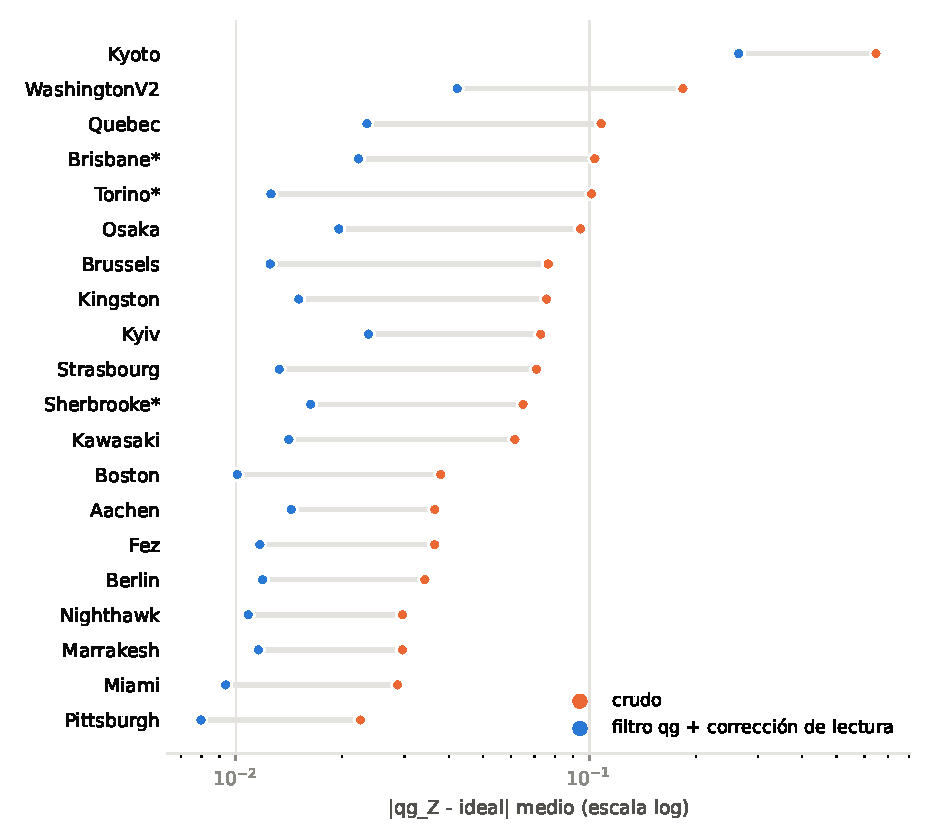
\includegraphics[width=0.78\linewidth]{fig_fleet_es.pdf}
\caption{Error de $\qZ$ crudo y filtrado (+ corregido por lectura) en veinte modelos de ruido de dispositivos
de IBM. Con asterisco: §137 (diez circuitos, 8000 disparos); el resto: §144 (cinco circuitos, 4000
disparos), dispositivos no usados antes.}
\label{fig:fleet}
\end{figure}

En los otros dieciocho \emph{fake backends} de al menos 100 qubits (dispositivos ECR, CZ y CX de 120 a 156
qubits), el filtro redujo el error 2{,}4--8{,}9 veces en cada uno de los diecisiete que corrieron
(Fig.~\ref{fig:fleet}; mediana crudo / filtro + lectura de 3{,}12). Aun así, las tres predicciones fallaron
tal como estaban escritas: un dispositivo se colgó (dos predicciones exigían los dieciocho), y filtro +
lectura fue lo más bajo en 10 de 17, y el filtro solo en los otros 7, donde los errores de lectura son chicos
y corregirlos agrega varianza. El cuelgue fue un error de la biblioteca: FakeCusco publica un qubit que
siempre lee 1, el transpilador ubicó el circuito ahí y la inversa de lectura era singular. Después del
arreglo, \texttt{best\_layout} esquiva ese qubit y baja el error filtrado de 0{,}098 a 0{,}021 (exploratorio).

\subsection{Predecir la fracción conservada y elegir qubits (§138, §141)}

Sobre diez ubicaciones por dispositivo, la predicción ordenó bien las ubicaciones (Spearman 0{,}94--0{,}98,
cumplida) y \texttt{best\_chain} conservó 6--17 puntos más de disparos que la ubicación por defecto de Qiskit
(cumplida), pero la predicción cruda quedó baja por 0{,}08--0{,}13 (fallida): ignoraba los disparos que
vuelven al sector. Con el piso de estado mezclado, agregado después de puntuar, el error es 0{,}023--0{,}041.
Para la QNN acoplada en anillo, \texttt{best\_chain} evaluó un circuito distinto del que corrió y conservó
menos disparos en dos dispositivos (§139); \texttt{best\_layout} lo corrige: nunca fue peor que la ubicación
por defecto y ganó 2{,}2 puntos donde eligió otra (§141, dos de tres predicciones cumplidas).

\subsection{Planificación de disparos (§143)}

Para un error objetivo de 0{,}02 el planificador pidió 3000--3400 disparos (0{,}8--0{,}9 segundos de
dispositivo); en 30 repeticiones el error del peor qubit fue 0{,}021--0{,}023 (cumplida). La predicción por
qubit quedó en promedio 1{,}4--1{,}6 veces baja (fallida): los qubits cerca de un polo ($|\qZ|>0{,}8$)
quedan subestimados 2{,}4--3{,}1 veces, porque el ruido aleja su $\qZ$ de $\pm1$; el plan lo fija el peor
qubit y aun así cumplió el objetivo.

\subsection{La QNN (§139--§141)}

\begin{table}[h]
\centering\small
\begin{tabular}{lccc}
\toprule
 & crudo & filtro & filtro + lectura\\
\midrule
\texttt{run\_qnn}, ubicación por defecto (§139) & 545 & 550 & 549\\
\texttt{run\_qnn}, \texttt{best\_chain} (§139) & 547 & 551 & 551\\
\texttt{run\_qnn}, \texttt{best\_layout} (§141) & 545 & 549 & 550\\
\texttt{SamplerQNN} de qiskit-machine-learning (§140) & 547 & 548 & --\\
\bottomrule
\end{tabular}
\caption{Decisiones correctas de 567 (189 entradas en cada uno de tres dispositivos; 555 sin ruido), 1000
disparos.}
\label{tab:qnn}
\end{table}

La plantilla de un solo trabajo coincide con los circuitos por entrada (550 contra 551, cumplida) y
qiskit-machine-learning reproduce el camino propio de la biblioteca (548, cumplida), pero el filtro recupera
solo 5--6 de las 10 decisiones que cuesta el ruido, y la corrección de lectura no cambia ninguna decisión
(Tabla~\ref{tab:qnn}). Corridas con la misma ubicación difieren hasta en dos decisiones, así que diferencias
de ese tamaño son ruido de muestreo. Al envolver la QNN en qiskit-machine-learning 0.9.1 apareció que, con un
\emph{pass manager} de dispositivo, \texttt{SamplerQNN} lee los bits medidos en las posiciones de los qubits
físicos de la ubicación, de modo que un circuito medido antes de transpilar lee cada disparo como 0 salvo
que su ubicación sea $[0,\dots,n-1]$; la biblioteca transpila por su cuenta y descarta la ubicación, y el
problema se informó al proyecto.

\subsection{Un espectro de PCA (§146)}

Cinco variables, 16 muestras de una gaussiana con desvíos estándar $(2{,}0;1{,}4;1{,}0;0{,}6;0{,}35)$ sobre
ejes aleatorios; espectro exacto $(0{,}640;0{,}203;0{,}122;0{,}023;0{,}011)$; un circuito por muestra (4 + 10
RBS, 26--28 compuertas nativas de dos qubits), 2000 disparos, en los tres dispositivos de §137 y los
dieciocho de §144, FakeCusco incluido tras la corrección. El error es
$L_1=\sum_k|\hat\lambda_k-\lambda_k/\sum\lambda|$. Las cuatro predicciones se cumplieron: sin ruido
$L_1=0{,}020$; corrieron los veintiuno y filtro + lectura quedó por debajo del crudo en todos; la razón
mediana crudo / filtro + lectura fue 4{,}6 (1{,}6--7{,}7); y los cinco autovalores salieron en orden en 18 de
21 (crudo 13, lectura 14, filtro 18). $L_1$ mediano: crudo 0{,}266, lectura 0{,}166, filtro 0{,}062, filtro
+ lectura 0{,}048. La estimación cruda está sesgada hacia arriba en todos los autovalores, porque los
disparos que salen del sector agregan excitaciones en todos los qubits (el espectro crudo suma más de 1); el
filtro elimina ese sesgo. Lo que queda es un aplanamiento del espectro que crece cuando baja la fracción
conservada: en FakeKyoto (15\% conservado) se pierde el orden, y en FakeBrisbane solo se invierten los dos
autovalores menores, que difieren en 0{,}012. La aceleración exponencial del PCA cuántico descansa en el
supuesto de que se dispone de copias de $\rho$~\cite{tang2021qpca}; este experimento no afirma nada sobre
ella.

\subsection{Simulación hamiltoniana y caminata cuántica (§147)}

\begin{figure}[h]
\centering
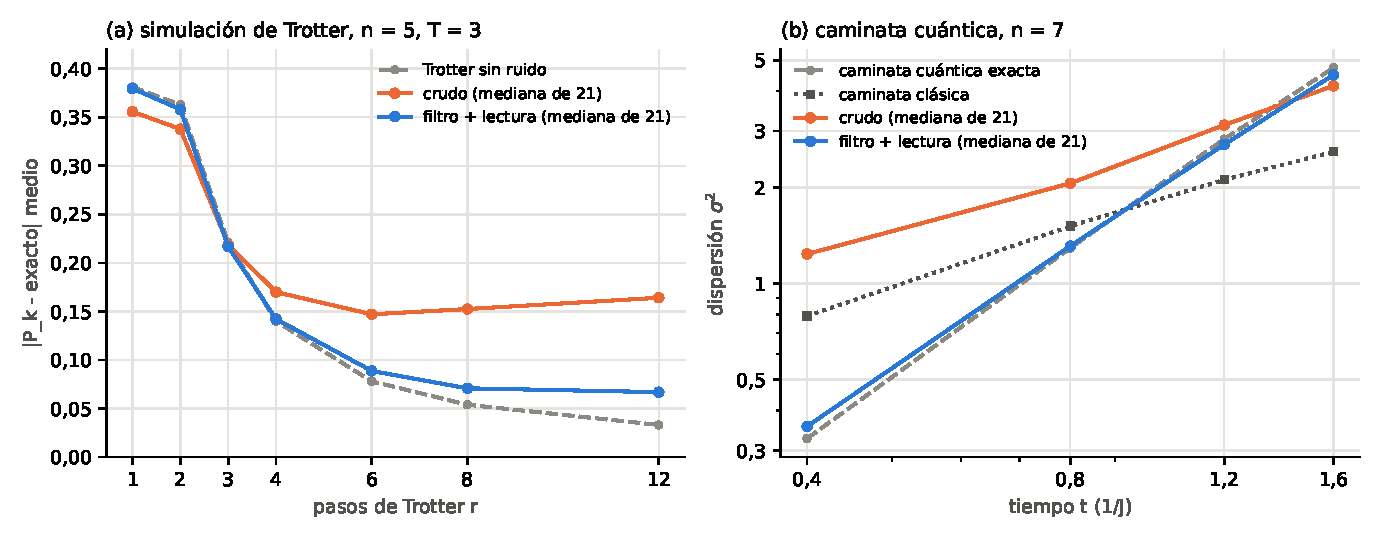
\includegraphics[width=\linewidth]{fig_trotter_es.pdf}
\caption{(a) Error de las ocupaciones simuladas en $T=3$ según el número de pasos de Trotter (cinco qubits,
campos aleatorios): más pasos bajan el error de Trotter (punteado) y agregan ruido; el filtro mantiene el
error en descenso hasta circuitos más profundos. (b) Dispersión de una caminata cuántica en siete qubits: los
datos crudos siguen una caminata clásica; los filtrados siguen la caminata cuántica exacta. Medianas sobre
veintiún modelos de ruido de dispositivos, 4000 disparos.}
\label{fig:trotter}
\end{figure}

Parte A: $n=5$, $J=1$, $h_k$ uniforme en $[-1,1]$, $T=3$, $r\in\{1,2,3,4,6,8,12\}$ (hasta 96 compuertas
nativas de dos qubits). Sin ruido el error de Trotter baja de 0{,}38 a 0{,}033; en un dispositivo tiene un
mínimo en algún $r^*$. Las tres predicciones se cumplieron (Figura~\ref{fig:trotter}a): con filtro + lectura
el mejor error es menor que el mejor error crudo en los veintiún dispositivos (1{,}6--2{,}8 veces, mediana
2{,}0), $r^*$ nunca es menor y es mayor en 16 de 21 (mediana 12 contra 8). En once dispositivos $r^*=12$, el
más profundo probado, así que el corrimiento es una cota inferior. Parte B: $h=0$, $n=7$, el caminante en el
qubit central, $t\in\{0{,}4;0{,}8;1{,}2;1{,}6\}$ con paso de Trotter 0{,}2; la dispersión exacta crece con
exponente 1{,}94 y una caminata clásica con la misma tasa con 0{,}85. Los datos crudos dan un exponente
mediano de 0{,}87: el ruido dispersa al caminante desde el principio y la caminata parece clásica
(Figura~\ref{fig:trotter}b). Con filtro + lectura el exponente mediano es 1{,}84, el crudo es menor en 20 de 21
(cumplida) y $\sigma^2$ queda dentro del 20\% del valor exacto en los cuatro tiempos en 15 de 21 (crudo:
ninguno; cumplida). El exponente llegó a 1{,}5 en 16 dispositivos, no en los 18 predichos (fallida): los cuatro
más ruidosos después de FakeKyoto dan 1{,}26--1{,}38, y en FakeKyoto (15\% de disparos conservados con 96
compuertas) la caminata se pierde.

\subsection{Excitaciones que interactúan (§148)}

\begin{table}[h]
\centering\small
\begin{tabular}{lccccc}
\toprule
excitaciones & crudo & lectura & filtro & filtro + lectura & crudo / filtro + lectura\\
\midrule
1 & 0{,}066 & 0{,}038 & 0{,}008 & 0{,}009 & 5{,}6 (2{,}4--14{,}4)\\
2 & 0{,}080 & 0{,}072 & 0{,}030 & 0{,}028 & 2{,}6 (1{,}1--3{,}8)\\
3 & 0{,}065 & 0{,}055 & 0{,}030 & 0{,}024 & 2{,}6 (1{,}0--4{,}6)\\
\bottomrule
\end{tabular}
\caption{Cadena XXZ, $n=6$, $V=2$, $T=2$: mejor error sobre el orden de Trotter (1, 2) y los pasos (1--8),
mediana sobre veintiún modelos de ruido de dispositivos; la última columna es la razón mediana y su rango
entre dispositivos.}
\label{tab:xxz}
\end{table}

Una excitación es el caso más fácil para el filtro y también es fácil clásicamente. Con $V=2$, campos
aleatorios en $[-0{,}5;0{,}5]$, $T=2$ y 1, 2 o 3 excitaciones que parten de los primeros qubits de una cadena de
seis, la dinámica es de muchos cuerpos. El beneficio del filtro baja de 5{,}6 veces con una excitación a
2{,}6 con dos y con tres (Tabla~\ref{tab:xxz}; se predijo que bajaría con cada excitación, cumplida apenas
entre dos y tres). Los sectores con más excitaciones conservan más disparos (0{,}49 contra 0{,}43 con 120
compuertas de dos qubits) pero ganan menos: más ruido cae dentro de un sector más grande (20 de 64 estados a
media ocupación, contra 6), donde el filtro no lo ve. Filtro + lectura fue lo mejor en 62 de los 63 pares
dispositivo--sector; en FakeKyoto a media ocupación no (0{,}238 contra 0{,}231), así que esa predicción falló.
El filtro volvió a correr a más profundidad el número óptimo de pasos de Trotter (61 de 63; mediana 8 o 6
contra 4), y Trotter de segundo orden fue mejor con dos excitaciones en 20 de 21 dispositivos (cumplida); con
tres, solo en 5, porque sus compuertas extra cuestan más de lo que ahorra su menor error de Trotter. Al armar
este experimento apareció que el pase del transpilador leía las X de preparación en el orden en que el DAG
lista las compuertas y podía informar mal el peso inicial; ahora toma una X como preparación cuando es la
primera operación en su qubit.

\subsection{Swap test, test de inversión y un clasificador por fidelidades (§149)}

Codificaciones de cinco qubits $v=(z,1)/|(z,1)|$ de iris versicolor y virginica ($z$: cuatro variables
estandarizadas; 15 flores de entrenamiento y 20 de prueba por clase); una flor de prueba va a la clase cuyo
prototipo (media normalizada de las codificaciones de entrenamiento) tiene mayor fidelidad, como
en~\cite{blank2020kernel}; 37 de 40 sin ruido. Cada test estimó 90 fidelidades (80 para el clasificador y 10
de un estado consigo mismo) en seis dispositivos, con 2000 disparos. Las cinco predicciones se cumplieron. El
test de inversión (12--16 compuertas nativas de dos qubits) con filtro + lectura llega a un error medio de
0{,}010--0{,}036, 3{,}8--11{,}2 veces menor que el crudo; el swap test (113--119 compuertas) llega solo a
0{,}089--0{,}239, 1{,}4--1{,}8 veces menor: su respuesta está en el qubit auxiliar, que el filtro no puede
proteger. El clasificador conserva su puntaje sin ruido con el test de inversión filtrado en todos los
dispositivos, y el swap test crudo obtiene 36--38: el ruido achica por igual las dos fidelidades de una flor,
así que la comparación sobrevive. El valor absoluto no: para un estado comparado consigo mismo ($F=1$) el
swap test crudo lee 0{,}20--0{,}65 y el test de inversión filtrado 0{,}92--1{,}00, que es lo que necesita un test
de igualdad. La corrida se dividió en un proceso por dispositivo después de que una corrida única superó el
límite de 2 horas del entorno, antes de ver ningún resultado.

\subsection{Errores ZZ coherentes que el filtro no debería ver (§145, §150)}

Los modelos de ruido de los dispositivos son canales incoherentes. A los diez circuitos de §137 en tres
dispositivos se agregaron dos errores coherentes que conservan el peso: una fase condicional mal calibrada,
RZZ($\varepsilon$) después de cada compuerta nativa de dos qubits sobre su par ($\varepsilon=0;0{,}05;0{,}10$ rad,
§145), y una interferencia ZZ permanente, $\exp(-i\theta ZZ/2)$ con $\theta=2\pi\nu t$ después de cada capa en
cada par acoplado de qubits usados, con $t$ tomado de las duraciones calibradas de las capas ($\nu=0;5;15$ kHz;
\texttt{add\_static\_zz}, §150). Las predicciones suponían que ambos eran invisibles para el filtro; cinco de las
siete fallaron. Los dos errores se filtran en parte: la fracción conservada bajó 0{,}009--0{,}020
($\varepsilon=0{,}10$) y hasta 0{,}023 (15 kHz), y el filtro eliminó el 32--60\% del error que agregó la
interferencia. Un término ZZ es diagonal en la base computacional, pero los qubits están en esa base solo
entre compuertas lógicas; dentro de la descomposición nativa de una compuerta XX+YY están rotados, y ahí ZZ
saca excitaciones del sector. Lo que pasa el filtro es modesto con estas intensidades: el error filtrado
creció 0{,}001--0{,}011 con el error de compuerta (4\% en los dispositivos ECR, 62\% en FakeTorino, donde la
descomposición con CZ expone más) y 0{,}003--0{,}009 (14--38\%) con 15 kHz de interferencia, menos en FakeTorino,
cuyos circuitos duran 2{,}1~$\mu$s contra 9--10~$\mu$s.

\section{Discusión}

Como herramienta de lectura, el filtro es robusto: en cada uno de los veinte modelos de ruido de
dispositivos de IBM bajó el error de $\qZ$ en un factor de 2{,}4 o más, y se combina con la corrección de
lectura y con la extrapolación a ruido cero. Cuál combinación es la mejor depende del dispositivo: la
corrección de lectura ayuda donde los errores de lectura son grandes y agrega varianza donde son chicos. La
calibración también dice, antes de gastar tiempo de dispositivo, cuántos disparos conservará el filtro, qué
qubits conservan más y cuántos disparos necesita una precisión objetivo.

Los límites son igual de claros. La ganancia en exactitud de clasificación es chica, porque las decisiones
del modelo están en su mayoría lejos del umbral; la estimación de espectros, donde la respuesta es un
conjunto de probabilidades y no una decisión, gana más (4{,}6 veces), y también la dinámica: el filtro permite que una simulación de Trotter use más
pasos y hace visible la dispersión balística de una caminata cuántica donde los datos crudos parecen
clásicos. Su beneficio es mayor con una excitación y se reduce a la mitad cuando las excitaciones
interactúan. Cuando la respuesta de un circuito está fuera de la simetría, como en el qubit auxiliar del
swap test, el filtro ayuda poco; una alternativa que conserve el peso, cuando existe, gana mucho más. Los errores que conservan el peso pasan el
filtro solo en parte, porque los qubits salen de la base computacional dentro de las compuertas nativas.
Dieciséis de las cuarenta y nueve predicciones fallaron tal como
estaban escritas, varias por el análisis y no por el filtro: una predicción que ignoraba los disparos que
vuelven, un modelo de error por qubit que ignoraba los polos y un experimento que exigía que corrieran todos
los dispositivos. Y todos los resultados son sobre modelos de ruido de dispositivos, que tratan los errores
de compuerta, relajación, desfase y lectura como canales independientes; la interferencia ZZ se agregó a mano
(§150) y no incluyen fugas ni deriva. El paso siguiente es una corrida en hardware.

\section*{Disponibilidad de código y datos}

Todo está en la biblioteca de código abierto qang (licencia MIT), versión 0.10.0 o posterior:
\url{https://github.com/Viny2030/qang}, \texttt{pip install qang}. El módulo es \texttt{qang.ibm} (con
\texttt{qang.qiskit\_ml}); cada sección tiene un script en \texttt{examples/} y su salida en
\texttt{examples/data/}; \texttt{docs/ibm\_quickstart.md} muestra el flujo de trabajo.

\begin{lstlisting}[language=Python]
from qang import ibm
t = transpile(qc, backend)                 # qc: conserva el peso, medido
res = Sampler(mode=backend).run([t]).result()[0]
ibm.ibm_qg(res, t, backend, weight=1)["filtered_readout"]
\end{lstlisting}

\bibliographystyle{unsrtnat}
\bibliography{../refs}

\end{document}
